\section{Computing Change Counts}

We now use the rungs of the versioning graph to quantify the amount of change by counting the number of changes in each change type.
Because VersOn has specific semantics for additions, invalidations, and modifications, the metric is also separated into three components.
The addition, invalidation, and modification counts for each transition up to Version 8.4.1 are presented in Table \ref{table:GCMD_main}.
\begin{table}
	\caption{Global Change Master Directory Keyword change counts.}
	\label{table:GCMD_main}
	\centering
	\begin{tabular}{@{}crrrr@{}}
		\toprule
		Transition&	Add&	Invalidate&	Modify&	Total\\
		\midrule
		June 12, 2012 to 7.0&	310&	9&	22&	341\\
		7.0 to 8.0&	503&	6&	79&	588\\
		8.0 to 8.1&	277&	28&	22&	327\\
		8.1 to 8.2&	53&	1&	26&	80\\
		8.2 to 8.3&	58&	0&	13&	71\\
		8.3 to 8.4&	53&	0&	1&	54\\
		8.4 to 8.4.1&	86&	13&	8&	107\\
		\bottomrule
	\end{tabular}
\end{table}
Modify changes are labeled as Moves to differentiate between types of modifications when discussing Version 8.5 in Section \ref{sec:85}.
Figure \ref{GCMDC1} plots the quantities and shows the individual change components as a bar chart and the total change as a line plot.
\begin{figure}[b]
	\centering
	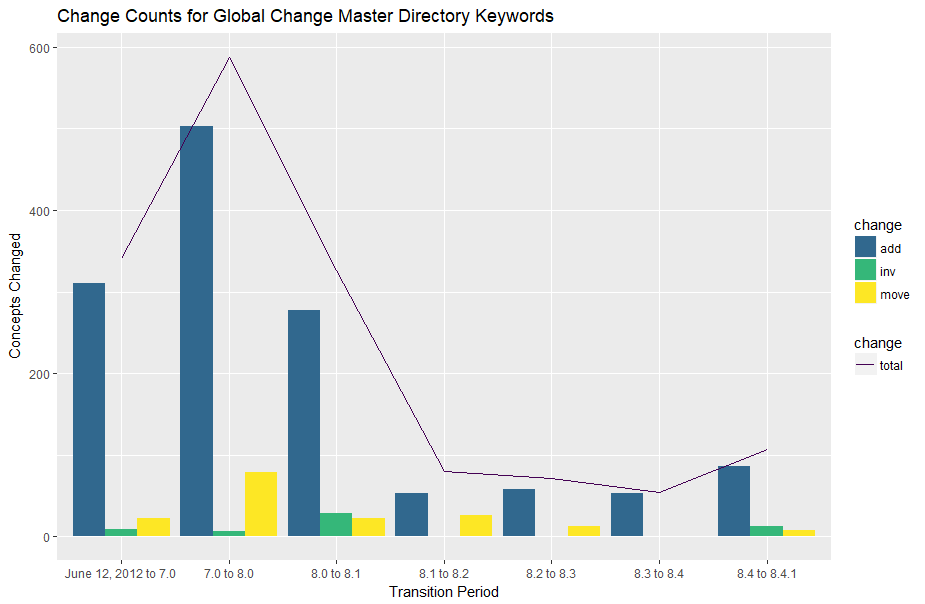
\includegraphics[scale=0.65]{GCMDChartShort_R.png}
	\caption{Add, Invalidate, and Modify counts from the beginning of the Keyword Management System to Version 8.4.1.}
	\label{GCMDC1}
\end{figure}
The plot demonstrates that dot-decimal identifiers show total summarized change as reflected by the total change.
Using VersOn, the change metric provides insight into the nature and components of change in the data set, capturing version change with greater precision.
From the bar chart, we can also see that additions dominate the kind of change in each interval.

A very clear discrepancy in the order of magnitude can be seen between major and minor version transitions except at the ``8.0 to 8.1" transition.
The publication of Version 7.0 and 8.0 both result in multi-hundred additions of concepts to the taxonomy.
Versions 8.2 to 8.4.1 only produced between 50 and 90 additions, an order of magnitude lower than major version changes.
There only exists a 33 addition difference separating changes induced by Version 8.1 and the changes created by Version 7.0.
Assuming the dot-decimal identifier assignment is correct, the quantitative cutoff between full and incremental releases lies around 300 addition changes.
The additions in ``8.4 to 8.4.1" in Figure \ref{GCMDC1} numbers almost a hundred, providing evidence that the trend of decreasing order of magnitudes may not continue as the granularity of the version identifier increases.



\subsection{GCMD Version 8.5} \label{sec:85}

While applying the URI based mapping method described in Section \ref{sec:vergraph} to Version 8.5, we collected a very alarming result.
In Table \ref{table:GCMD_8_5}, `URI Based' shows the number of additions and invalidations at about the size of the entire GCMD Keywords data set.
\begin{table}
	\caption{Difference in Version 8.5 mapping methods.}
	\label{table:GCMD_8_5}
	\centering
	\begin{tabular}{@{}crrrr@{}}
		\toprule
		Mapping Method&	Add&	Invalidate&	Move&	Modify\\
		\midrule
		URI Based&	3097&	3031&	0&	0\\
		Bridged&	68&	2&	22&	3007\\		
		Silent&	68&	2&	22&	0\\
		\bottomrule
	\end{tabular}
\end{table}
In addition, no modifications are revealed, and even the root node "Science Keywords" has been invalidated, meaning the GCMD Keywords group had removed and replaced the entire taxonomy.
Further investigation of the root word reveals that the name space for the keywords has changed from \mintinline{HTML}{http} to \mintinline{HTML}{https}.
To provide context, National Aeronautics and Space Administration (NASA) mandated a transition to secure protocols, and the group changed the name space to ensure the URIs remained resolvable.
Since the URIs are lexically unique, the new name space means new URIs no longer refer to the same object after the protocol change.
Because the keyword identifiers no longer match, the mapping approach results in the total invalidation of keywords from 8.4.1 and the addition of keywords from 8.5.
The dot-decimal identifier for the transition from Version 8.4.1 to 8.5 does not match the number of changes in the versioning graph.

Changing the mapping method to account for the new namespace provides a pathway to compare the perceived change by the producer as evidenced by the version identifier with the change distance in the versioning graph.
To do this, the mapping treats identifiers with \mintinline{html}{http} and \mintinline{html}{https} the same, revealing keywords actually added, invalidated, and moved.
The code breaks apart the UUID from the URI and uses the prior namespace or current namespace, respectively.
Differences in change distance become much clearer after controlling for the altered name space in Figure \ref{GCMDC2} under the label `Bridged'.
\begin{figure}%[b]
	\centering
	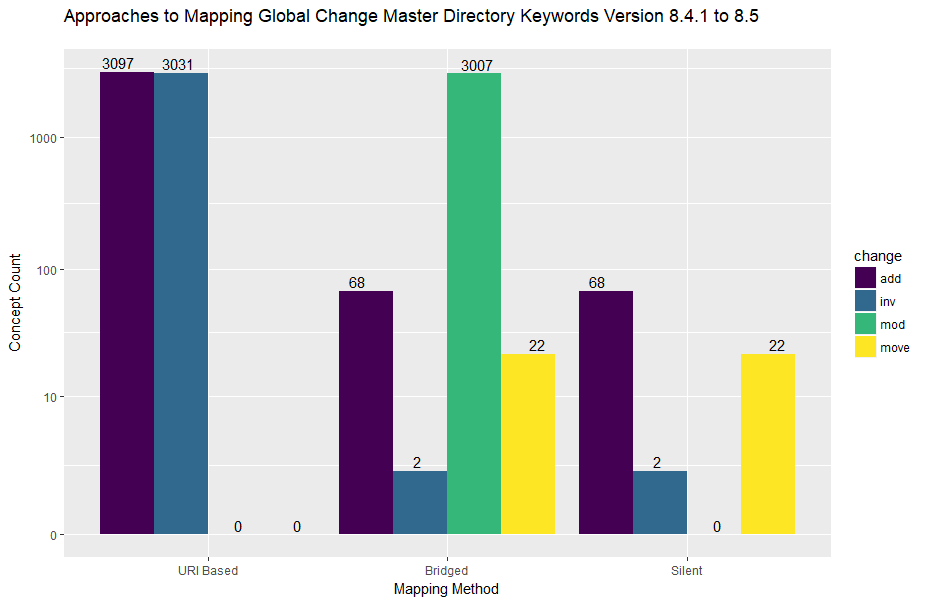
\includegraphics[scale=.65]{GCMD8_5_R.png}
	\caption{Add, Invalidate, and Modify counts using different methods of mapping identifiers in Global Change Master Directory Keywords Version 8.4.1 to 8.5.}
	\label{GCMDC2}
\end{figure}
The Silent method ignores the change in namespace by considering concepts with matching UUIDs as unchanged.
Only the Silent method follows the previous minor release trend of being addition dominated and having less than a hundred additions.



